\documentclass[../main.tex]{subfiles}
\begin{document}
\paragraph{Offline solutions}\label{par:burgers_fom}

Due to the nonlinearity of the advection term the assembly of the FOM will now require some further steps.
In particular the discretisation of the operator $\mathcal{L}_{\mu}$ in $\mathbb{R}^{N_{h}}$ would not lead to a linear operator $\boldsymbol{M}$ because $\mathcal{L}_{\mu}$ is not linear.

\begin{figure}[H]
    \centering 
    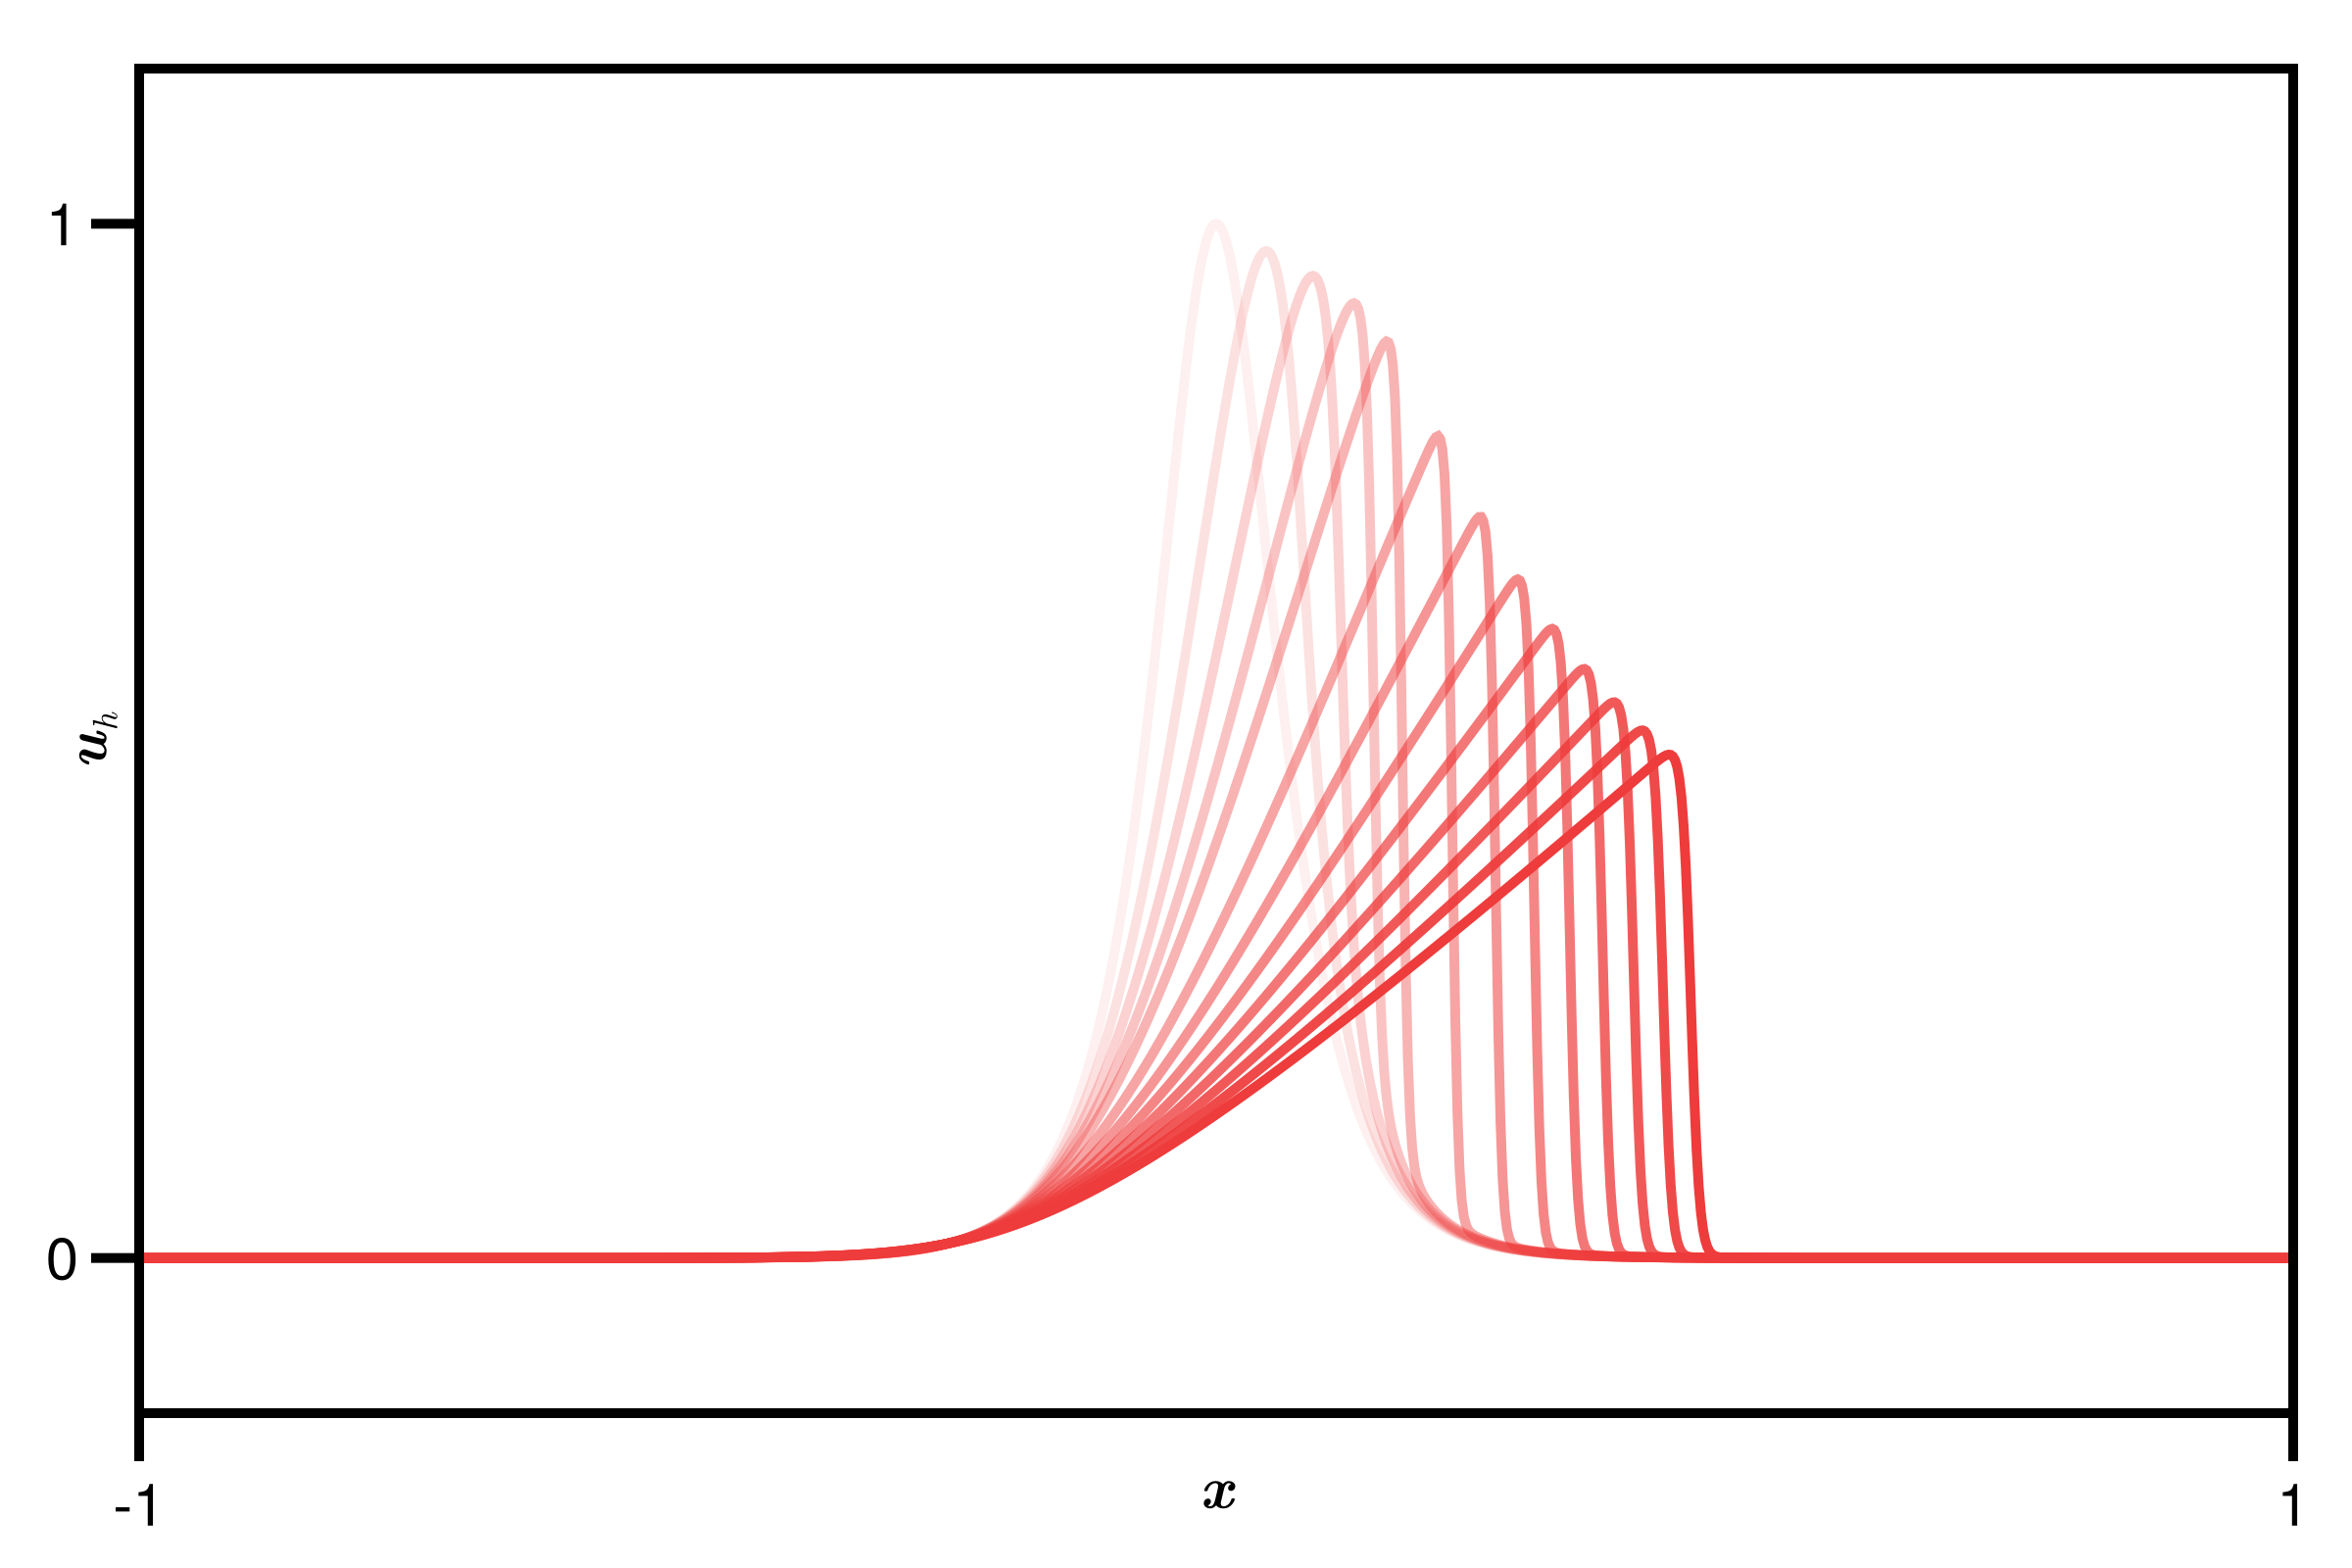
\includegraphics[keepaspectratio, width=0.7\textwidth]{../figures/fig:burgers_fom.png}
    \caption{Some snapshots of the FOM of \eqref{eq:burgers} at different timesteps (lighter colors indicate older timesteps).}
    \label{fig:burgers_fom}
\end{figure}

The high dimensional dynamical system reads

\begin{equation*}
        \dot{\boldsymbol{u}}_{h} = \boldsymbol{M}^{-1}(\boldsymbol{D}\boldsymbol{u}_{h} + \boldsymbol{N}(\boldsymbol{u}_{h})) = \underbrace{\boldsymbol{M}^{-1}\boldsymbol{D}}_{\boldsymbol{L}}\boldsymbol{u}_{h} + \underbrace{\boldsymbol{M}^{-1}\boldsymbol{N}(\boldsymbol{u}_{h})}_{\boldsymbol{c}(\boldsymbol{u}_{h})}\,,
\end{equation*}

where $\boldsymbol{D}$ discretises the (linear) diffusion term of \eqref{eq:burgers} and the $\boldsymbol{N}$ discretises the nonlinear advection term

\begin{equation*}
        \boldsymbol{N}(\boldsymbol{u}_{h})=\Bigg[N_{j}(\boldsymbol{u}_{h}) = \int_{\Omega}^{}\varphi_{j}\Bigg(\sum_{k=1}^{N_{h}}u_{k}\varphi_{k}\Bigg)\Bigg(\sum_{k=1}^{N_{h}}u_{k}\newprime{\varphi}_{k}\Bigg)\Bigg]_{j=1,\dots,N_{h}}\,,
\end{equation*}

which is clearly quadratic in $\boldsymbol{u}_{h}$.
The FOM is retrieved by applying Euler implicit time-stepping \eqref{eq:euler_implicit} to the high-dimensional nonlinear system

\begin{equation}\label{eq:burgers_fom}
     \delta t \boldsymbol{N}(\boldsymbol{u}_{h}(t_{n+1})) + (\delta t \boldsymbol{M}^{-1}\boldsymbol{D}-\boldsymbol{I})\boldsymbol{u}_{h}(t_{n+1}) - \boldsymbol{u}_{h}(t_{n}) =: \boldsymbol{G}(\boldsymbol{u}_{h}(t_{n+1})) = \boldsymbol{0}_{\mathbb{R}^{N_{h}}} \,.
\end{equation}

Notice how \eqref{eq:burgers_fom} is an implicit nonlinear system of equations in $\mathbb{R}^{N_{h}}$ as opposed to e.g. the high-dimensional linear system we derived in \eqref{eq:heat_fom} for a linear parabolic model. 
This is solved iteratively by root-finding algorithms s.a. Newton-Raphson or gradient descent.
We do this for a single diffusion value $\mathcal{P}=\{0.01\}$ and for a time horizon $T=1$.
The snapshot matrix $\boldsymbol{X}$ will thus contain the $N_{f}=10^{3}$ transient solutions propagated from the localised IC.
Some of these FOM snapshots are depicted below in Figure \ref{fig:burgers_fom}.

\end{document}
